% CSE 5999 Progress Report #2 -- Brian Zhou
% IEEE CVPR template (camera-ready mode so the author is shown), as in Report #1.
% Drafted with Claude (Anthropic), 1 Nov 2026, from the project's own files
% (PROGRESS.md, DECISIONS_LOG.md, the IGARSS draft, the Gate 2 results).
\documentclass[10pt,twocolumn,letterpaper]{article}

\usepackage[T1]{fontenc}
\usepackage[pagenumbers]{cvpr}

\usepackage{graphicx}
\usepackage{amsmath}
\usepackage{amssymb}
\usepackage{booktabs}
\usepackage[breaklinks,colorlinks]{hyperref}
\usepackage[capitalize]{cleveref}
\crefname{section}{Sec.}{Secs.}
\Crefname{section}{Section}{Sections}
\Crefname{table}{Table}{Tables}
\crefname{table}{Tab.}{Tabs.}

\def\cvprPaperID{*****}
\def\confName{CSE 5999}
\def\confYear{2026}

\begin{document}

\title{Progress Report \#2: Does Remote Sensing Beat the Trail Map?\\Predicting Hiking Speed in Unseen Regions}

\author{Brian Zhou\\
Washington University in St.\ Louis\\
{\tt\small zhou.n@wustl.edu}\\
{\small CSE 5999 Independent Study, Fall 2026 \;$\cdot$\; Mentors: Danni Beaulieu, Tianyi Gao \;$\cdot$\; Advisor: Prof.\ Nathan Jacobs}
}
\maketitle

%-----------------------------------------------------------------------------
\begin{abstract}
I predict hiking speed on 50\,m trail segments from OpenStreetMap (OSM) GPS traces and ask what corrects Tobler's 1993 hiking function in regions a model has never seen: OSM trail tags or terrain measured from elevation models. Since Report~\#1 the dataset grew from a three-region sample to 290{,}640 walking traversals from about 2{,}000 hikes in 17 North American mountain regions. Holding out one region at a time and scoring full predictive distributions (CRPS), Tobler's function is 12.5\% worse than a refitted slope curve; terrain improves on that curve by 2.1--2.8\% and beats the tags in 16 of 17 regions. A new model, \emph{learned Tobler}, keeps Tobler's curve but lets a small network set its constants from terrain. It ties gradient-boosted trees on the shared spread rule and beats them by about 0.6 points with its own uncertainty, while staying interpretable.
\end{abstract}

%-----------------------------------------------------------------------------
\section{Project Plan and Scope}
\label{sec:plan}

\paragraph{Problem.} Tobler's function~\cite{tobler1993}, $v = 6\exp(-3.5\,|s+0.05|)$ km/h for slope $s$, is still the default walking-speed model in GIS, but it was fit to a few published figures, not to observed hikes. Maps record trail attributes (OSM \texttt{surface}, \texttt{sac\_scale}) only patchily, while airborne lidar now measures terrain almost everywhere in the US. The question is whether \emph{remotely sensed terrain can replace the trail attributes a map lacks}, judged where it matters: in regions the model never saw. The design is unchanged from the plan: arms that predict the same target and differ only in their inputs (Tobler, slope only, tags, terrain, tags + terrain).

\paragraph{Goals.} \emph{Minimum} (on track): the frozen four-arm comparison in unseen regions with calibrated predictions, written up as a four-page IGARSS 2027 paper (deadline 11 January 2027; a complete first draft exists). \emph{Maximum}: in addition, an interpretable learned-Tobler model that is as accurate as boosted trees (now reached, \cref{sec:results}), an aerial-imagery arm (NAIP) tested for transfer to unseen regions, and a cleaned public release of the segment dataset if the mentors approve it.

\paragraph{Scope changes since Report~\#1, and why.}
(i)~\emph{One region $\to$ 17 regions pooled.} Gate~1 found only 54--82 hikes per sample region, too few for one region. Pooling 17 regions gives about 2{,}000 hikes and makes the stronger test possible: leave one region out.
(ii)~\emph{The headline metric is transfer.} Every result is reported for five hold-outs: new hikes, new hikers, new 10\,km squares, unseen regions, and unseen regions with unseen hikers.
(iii)~\emph{Vegetation and satellite embeddings are minor.} Lidar vegetation added little, and AlphaEarth embeddings helped mainly inside training regions (they mostly identify the place), so both are one sentence in the paper instead of arms.
(iv)~\emph{New model.} The planned terrain-dependent Tobler backbone is now built as learned Tobler (\cref{sec:approach}); the paper's numbers stay frozen and it is reported alongside them.
(v)~\emph{Imagery} moves to week~12 (9--15 Nov), decided at Gate~2 on 6 Nov.

%-----------------------------------------------------------------------------
\section{Related Work Update}
\label{sec:related}

Report~\#1 covered the speed-from-overhead-data work of the Jacobs group~\cite{hadzic2020rasternet,workman2020dynamic,workman2024probabilistic}, pedestrian travel rates~\cite{asako2024hikingtte,campbell2022variability} and the lidar-based STRIDE model~\cite{campbell2024stride,cutler2026machine}. The papers below are new since then: the work behind the learned-Tobler design and the imagery plan.

\paragraph{Predicting uncertainty.} Kendall and Gal~\cite{kendall2017uncertainties} (NeurIPS 2017) separate \emph{aleatoric} noise, which a network can predict per input by outputting a variance and training with the likelihood, from \emph{epistemic} uncertainty. My model's $\sigma$ output is exactly their heteroscedastic aleatoric head; I use a Student-$t$ instead of a Gaussian because GPS glitches and missed stops give heavy tails. I score with CRPS, a proper scoring rule~\cite{gneiting2007strictly}.

\paragraph{Starting from a known model.} ControlNet~\cite{zhang2023controlnet} (ICCV 2023) adds a trainable branch to a pretrained diffusion model through ``zero convolutions'', so training starts exactly at the pretrained model and only learns departures from it. Learned Tobler uses the same trick: its output layer starts at zero with biases equal to the refitted slope curve, so the untrained model \emph{is} the baseline (to $3\times10^{-7}$), and any gain is a gain over slope alone.

\paragraph{Evaluating on unseen domains.} Gulrajani and Lopez-Paz~\cite{gulrajani2021lost} (ICLR 2021) show that domain-generalization claims depend on how models are selected, and that selection must not use the test domain. My leave-one-region-out split follows this: early stopping and the spread used for scoring come from held-in hikes only, and clipping and scaling are fitted on training rows.

\paragraph{The tree baseline.} The trees arm is scikit-learn's histogram-based gradient boosting, inspired by LightGBM~\cite{ke2017lightgbm} (NeurIPS 2017); learned Tobler must match it to be worth its interpretability.

\paragraph{Imagery encoders.} SatlasPretrain~\cite{bastani2023satlaspretrain} (ICCV 2023) is a large remote-sensing dataset with pretrained Swin backbones, including ones for 0.5--2\,m aerial imagery such as NAIP. Its frozen aerial encoder is my first choice for trail-centred image chips in week~12, because it is open and trained at the right resolution; location encoders are ruled out because they would leak the held-out region.

%-----------------------------------------------------------------------------
\section{Proposed Approach}
\label{sec:approach}

\paragraph{Target and splits.} Each row is one hiker walking one 50\,m segment; the target is $y=\ln$(speed in km/h). Folds split by outing, hiker, 10\,km block, region (17 folds) and region-with-new-hikers. Inside each fold, training outings are split 70/15/15 into \emph{fit} (learn), \emph{stop} (early stopping) and \emph{cal} (spread for scoring); the test fold is never touched.

\paragraph{Learned Tobler.} Tobler's curve with a rounded peak,
\begin{equation}
\mu = a - k_{\pm}\big(\sqrt{(s+s_0)^2+e^2}-e\big),\quad y\sim t_{5}(\mu,\sigma),
\end{equation}
where $k_{+}$ applies uphill and $k_{-}$ downhill of the peak. A multilayer perceptron sees only terrain (12 measures of the segment from the 1\,m and 5\,m elevation models, such as pitch steepness, step variability, hidden climbing and cross-slope, plus 7 missing-value flags; 19 inputs $\to$ 32 $\to$ 32 $\to$ 5, SiLU, 1{,}861 weights) and outputs the five constants $a$, $k_{+}$, $k_{-}$ (softplus, so speed always falls away from the peak), $s_0$ and $\log\sigma$. Slope enters only through the formula, so every prediction is still a Tobler-shaped curve whose constants can be read off. Inputs are clipped to the training rows' 0.1--99.9th percentiles and standardized. Training: Adam (learning rate $10^{-3}$, batch 2{,}048), Student-$t$ negative log-likelihood ($\nu=5$), early stopping on the stop rows (patience 5, at most 60 passes), three seeds. Code: \texttt{exercises/week10\_learned\_tobler/} (\texttt{learned\_tobler.py}, \texttt{run\_all.py}, \texttt{gate2\_summary.py}).

\paragraph{Scoring.} CRPS in log speed, as skill over the refitted slope curve: $100(1-\sum\mathrm{CRPS}/\sum\mathrm{CRPS}_{\text{ref}})$. Learned Tobler gets two scores: (a)~its centre with the same spread rule as every model in the paper (quantiles of the cal residuals), and (b)~its own Student-$t$. Uncertainty is a 2{,}000-draw bootstrap over outings, hikers or regions, with paired differences against the trees.

\paragraph{Next: imagery (week 12).} Track~A joins Clay v1.5's precomputed NAIP embeddings (one 1{,}024-number vector per 154\,m chip; about 6.5\,GB for our 805 quarter quads) and reduces them to 16 numbers by PCA fitted per fold. Track~B, if A is promising, cuts 96\,m chips centred on each of the 173{,}444 trail spots from NAIP on Microsoft Planetary Computer and embeds them with a frozen Satlas encoder~\cite{bastani2023satlaspretrain} on the cluster's CPUs. Both reuse the same folds and scoring; success means terrain + imagery beats terrain alone in unseen regions with the 95\% interval above zero.

%-----------------------------------------------------------------------------
\section{Data and Resources}
\label{sec:data}

\paragraph{Segments.} 290{,}640 walking traversals of 50\,m trail segments from public OSM GPS traces (identifiable and trackable traces, which keep timestamps), about 2{,}000 outings by 881 hikers in 17 regions (16 in the US, one in Canada). Traces are cleaned, stop-filtered and map-matched to the OSM trail graph. There are no human labels: speed comes from the timestamps; OSM tags (\texttt{sac\_scale}, \texttt{surface}, \texttt{trail\_visibility}) are attributes, present on only part of the trail length.

\paragraph{A real example.} The Gulfside Trail near Mt Washington, NH, is tagged \texttt{highway=path}, \texttt{sac\_scale=mountain\_hiking}, \texttt{surface=ground}. On smooth trail a segment's 5\,m pitches vary by about 0.015 in grade (pitch SD); on rock steps and stairs by about 0.17. Elevation errors at fixed steep spots, such as the cliff edge at Taft Point in Yosemite and the stairs at Lower Twin Falls, produced 1{,}065 segments with a 5\,m pitch above 100\%; inputs are now clipped (decisions \#121--\#122).

\paragraph{Terrain.} USGS 3DEP elevation models at 1\,m (lidar) and 5\,m, plus NLCD tree canopy; NAIP (0.6\,m, 0.3\,m in three states) covers the 16 US regions.

\paragraph{Platform.} Python (PyTorch, scikit-learn) on my laptop (Apple M4, 16\,GB): all learned-Tobler runs, 5 splits $\times$ 3 seeds, take about 6 minutes on its CPU. Data processing runs on the McKelvey Engineering cluster (Slurm, CPU only), where the large data stay. Resources are adequate; imagery Track~B needs about 25--35\,GB of tile reads and PyTorch installed on the cluster.

%-----------------------------------------------------------------------------
\section{Results So Far}
\label{sec:results}

\paragraph{Implemented.} The full pipeline from GPS traces to scored models: download, cleaning, stop filtering, map-matching, 50\,m segments, terrain and tag features, the evaluation harness with all five splits, the four arms, and a first full IGARSS draft (4 pages). Since the last report I also ran the log-linear diagnostic (week~9), built and trained learned Tobler (weeks 10--11), and hand-checked 20 detected stops (first pass; a second pass comes before scoring).

\paragraph{Main comparison (frozen for the paper).} Holding out one region at a time, Tobler's fixed constants are 12.5\% worse than a refitted slope curve. Terrain improves CRPS by 2.1--2.8\% in unseen regions and beats OSM tags in 16 of 17 regions; tags add 0.4--0.9\%. For the same hiker on the same trail, descending is 8--23\% faster than climbing, not the 42\% Tobler implies.

\begin{table}[t]
\centering
\footnotesize
\setlength{\tabcolsep}{3pt}
\begin{tabular}{@{}lrccc@{}}
\toprule
Hold-out (unit) & units & Trees & LT (a) & LT (b) \\
\midrule
New hikes (outing) & 1{,}992 & 3.22 & 3.19 & \textbf{3.77} \\
New hikers & 881 & 3.19 & 3.07 & \textbf{3.36} \\
New 10\,km squares & 1{,}992 & 2.83 & 2.90 & \textbf{3.50} \\
Unseen region & 17 & 2.79 & 3.01 & \textbf{3.37} \\
Unseen region + hikers & 17 & 2.42 & 2.55 & \textbf{3.05} \\
\bottomrule
\end{tabular}
\caption{CRPS skill (\%) over the refitted slope curve, 289{,}679 test segments, learned Tobler (LT) averaged over 3 seeds. (a) shares the trees' spread rule; (b) uses LT's own Student-$t$. (a)$-$Trees spans zero in every hold-out (a tie); (b)$-$Trees is $+0.55$ to $+0.66$ points for new hikes, new squares and unseen regions, with 95\% intervals above zero.}
\label{tab:gate2}
\end{table}

\paragraph{Learned Tobler (\cref{tab:gate2}).} With the same spread rule it ties the trees in all five hold-outs ($-0.12$ to $+0.22$ points). With its own uncertainty it is ahead. Its 90\% intervals contain 89.4--89.9\% of test segments in every hold-out (the North Shore is lower, about 82\%, for every model). Across seeds the score moves by at most 0.24 points. What it learned (\cref{fig:constants}): $k$ stays between about 1.9 and 2.7, never Tobler's 3.5, and the peak speed falls from 4.5 to 3.6\,km/h from smooth to steppy trail.

\begin{figure}[t]
\centering
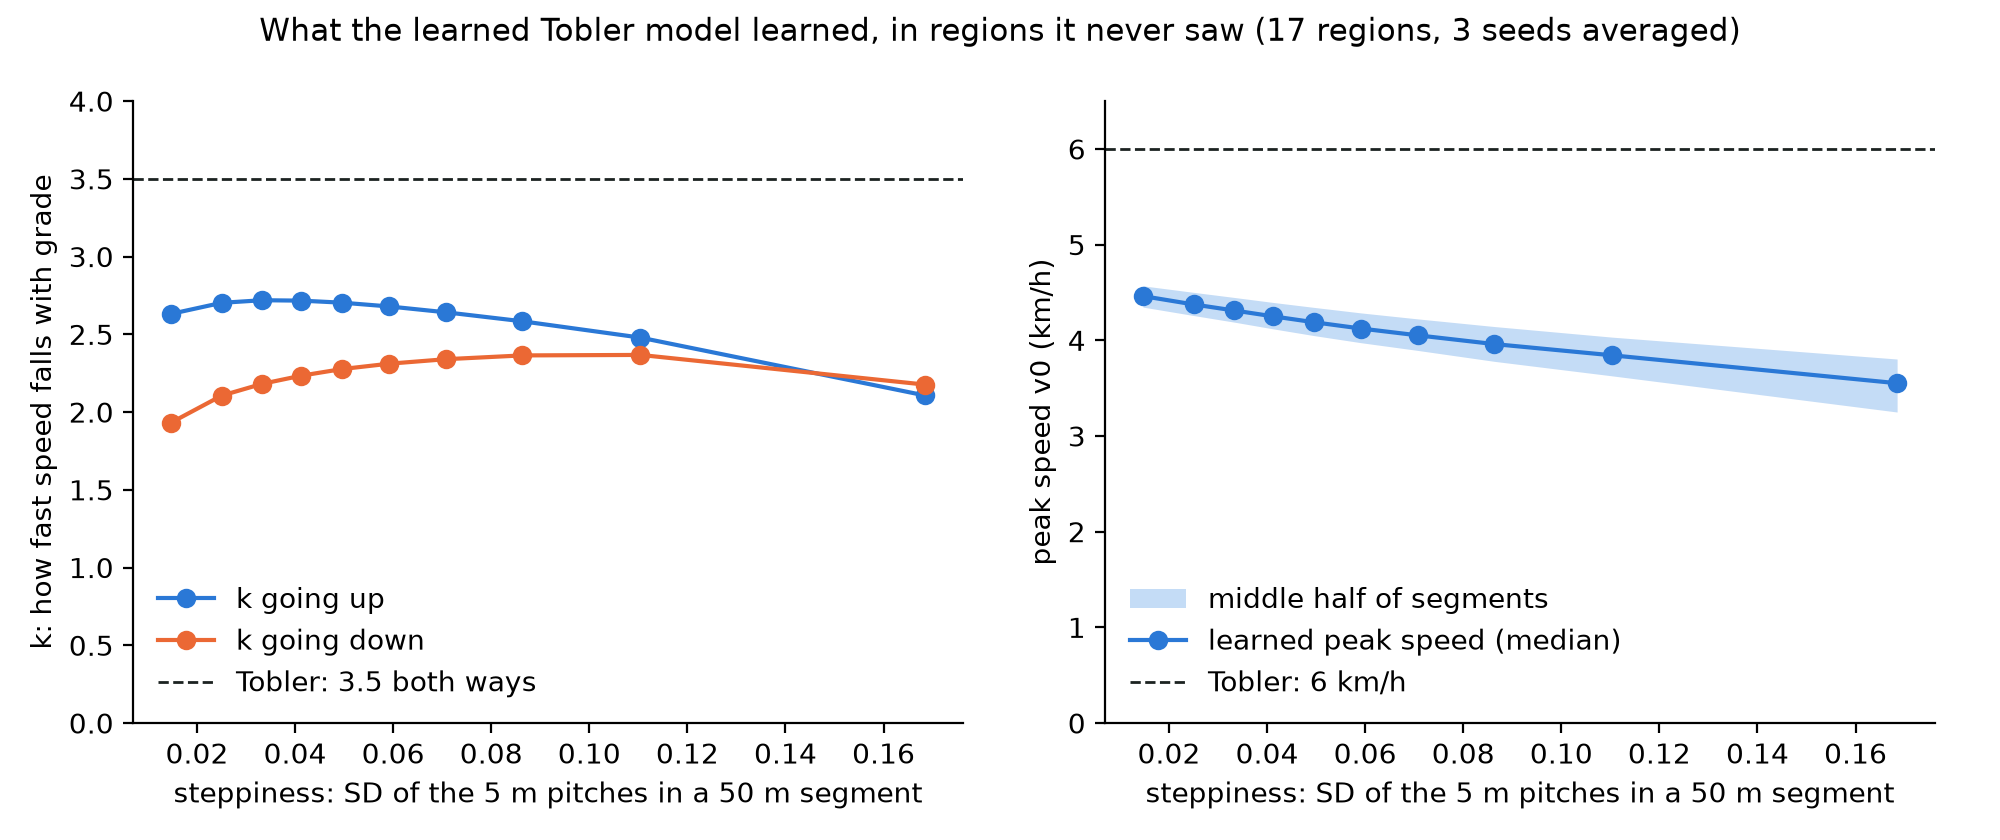
\includegraphics[width=\linewidth]{figures/fig_constants.png}
\caption{Learned-Tobler constants in unseen regions against steppiness (SD of the 5\,m pitches in a segment), medians of ten equal-count bins. Left: $k$ uphill and downhill. Right: peak speed. Dashed: Tobler.}
\label{fig:constants}
\end{figure}

%-----------------------------------------------------------------------------
\section{External Assistance and Collaboration}
\label{sec:help}

My PhD mentors, Danni Beaulieu and Tianyi Gao, meet with me weekly. Danni set the semester plan, its gates and the arm design, shared the lab's OSM data, and asked for the learned-Tobler setup specification; Tianyi co-mentors the project in our meetings. Prof.\ Nathan Jacobs is my faculty advisor. I use Claude (Anthropic), an AI assistant, extensively: it wrote most of the data-processing, modeling and evaluation code, including most blanks in my weekly exercises, ran the downloads and experiments, drafted the IGARSS paper and the write-ups, and drafted this report from the project's files. I ran and checked the exercises, labeled the stop check, and reviewed the results and text, and I am responsible for them. Data come from OSM contributors, USGS 3DEP, MRLC, and Microsoft Planetary Computer.

%-----------------------------------------------------------------------------
\section{Reservations and Questions}
\label{sec:questions}

\begin{itemize}\setlength\itemsep{1pt}
\item \textbf{Is the learned-Tobler win fair?} Its edge comes from its own learned spread, and the trees had no learned spread in this comparison (an earlier attempt to give them one did not help). Should the paper claim ``as accurate and interpretable'' rather than ``better''?
\item \textbf{Elevation glitches.} Clipping fixed the model, but the released data should cap pitches; are the paper's binned models really unaffected everywhere?
\item \textbf{Stops.} My first hand-check of 20 stops was rushed; the second pass decides whether the stop rule needs tuning.
\item \textbf{Will imagery transfer?} A 154\,m Clay chip shows the landscape, not the trail, so it may only identify the place, as AlphaEarth did. Trail-centred chips (Track~B) are the real test but cost 3--4 days.
\item \textbf{Hardest part now:} turning the draft into my own words by week~13 while finishing imagery, and the data-release decision.
\end{itemize}

{\footnotesize
\setlength{\itemsep}{0pt}\setlength{\parskip}{0pt}
\bibliographystyle{ieee_fullname}
\bibliography{refs}
}

\end{document}
